\chapter{Customização}

Algumas opções de customização estão disponíveis para o usuário do InVesalius. Elas
são apresentadas a seguir.

\section{Menu de ferramentas}

Para ocultar/exibir o menu lateral de ferramentas, clique sobre o botão que a figura
\ref{fig:layout_full_original} ilustra.

\begin{figure}[!htb]
\centering

\includegraphics[scale=0.5]{../user_guide_figures/icons/layout_full_original.png}
\caption{Atalho para ocultar/exibir menu lateral de ferramentas}
\label{fig:layout_full_original}
\end{figure}

Com o menu ocultado, amplia-se a área da janela do InVesalius disponível para a
visualização das imagens, conforme mostra a figura \ref{fig:closed_tool_menu}.

\begin{figure}[!htb]
\centering
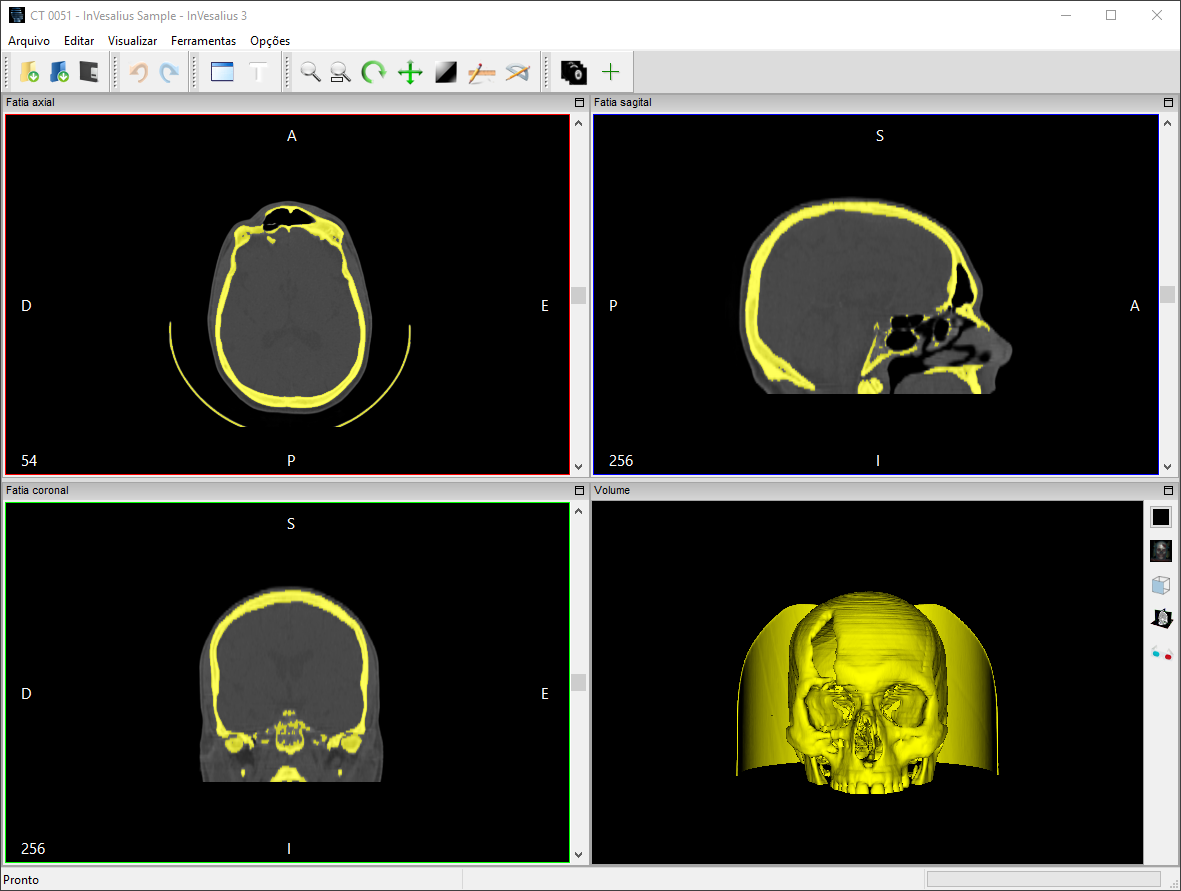
\includegraphics[scale=0.4]{../user_guide_figures/invesalius_screen/window_mpr_not_painels_pt.png}
\caption{Menu lateral ocultado}
\label{fig:closed_tool_menu}
\end{figure}

\newpage

\section{Posicionamento automático de volume/superfície}

Para acertar automaticamente a posição de visualização de um volume ou superfície,
pode-se clicar sobre o ícone apresentado na figura \ref{fig:3d_automatic_position}
(localizado no canto inferior direito da tela do InVesalius) e escolher uma das
opções de visualização disponíveis.

\begin{figure}[!htb]
\centering
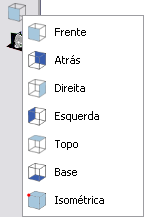
\includegraphics[scale=0.45]{../user_guide_figures/invesalius_screen/3d_automatic_position.png}
\caption{Opções de posição para visualização}
\label{fig:3d_automatic_position}
\end{figure}

\section{Cor de fundo da janela de volume/superfície}

Para alterar a cor de fundo da janela de volume/superfície, clique no atalho que a figura
\ref{fig:button_select_color_2} mostra. O atalho também está localizado no canto inferior
direito da tela do InVesalius.

\begin{figure}[!htb]
\centering

\includegraphics[scale=0.8]{../user_guide_figures/invesalius_screen/colour_button.png}
\caption{Atalho para cor de fundo da janela de volume/superfície}
\label{fig:button_select_color_2}
\end{figure}

Uma janela para seleção de cor se abre, como aparece na figura \ref{fig:color_window_background}.
Após isso, basta clicar sobre a cor desejada e, em seguida, clicar em \textbf{OK}.

\begin{figure}[!htb]
\centering
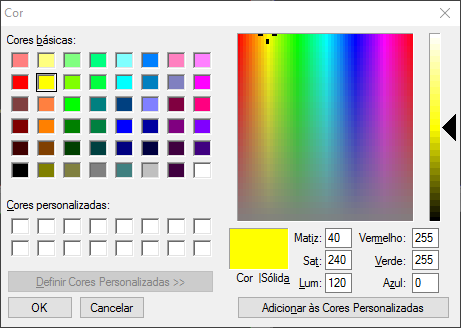
\includegraphics[scale=0.6]{../user_guide_figures/invesalius_screen/surface_select_color_windows_so_pt.png}
\caption{Seleção de cor de fundo}
\label{fig:color_window_background}
\end{figure}

A figura \ref{fig:background_color} mostra um exemplo dessa janela com a cor de fundo alterada.

\begin{figure}[!htb]
\centering
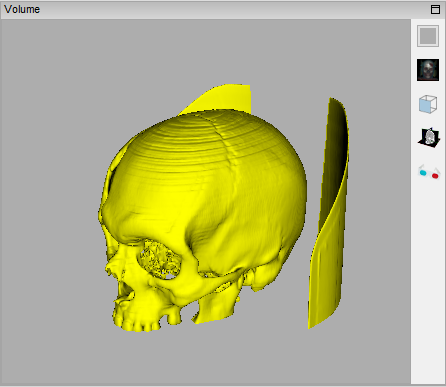
\includegraphics[scale=0.7]{../user_guide_figures/invesalius_screen/3d_background_changed.png}
\caption{Cor de fundo alterada}
\label{fig:background_color}
\end{figure}

\newpage

\section{Exibir/ocultar textos em janela 2D}

Para exibir ou ocultar os textos que aparecem nas janelas de imagens 2D, clique no atalho
exibido na figura \ref{fig:text}, localizado na barra de ferramentas.

\begin{figure}[!htb]
\centering

\includegraphics[scale=0.7]{../user_guide_figures/icons/text.png}
\caption{Atalho para exibir ou ocultar texto}
\label{fig:text}
\end{figure}

As figuras \ref{fig:text_on} e \ref{fig:text_off} ilustram, respectivamente, a exibição
dos textos habilitada e desabilitada.

\begin{figure}[!htb]
\centering
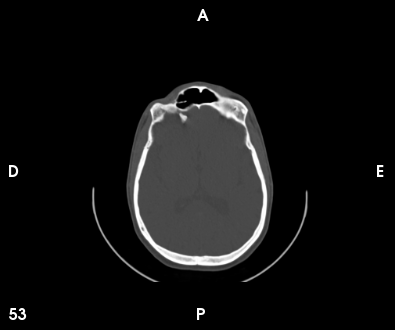
\includegraphics[scale=0.5]{../user_guide_figures/invesalius_screen/text_on.png}
\caption{Exibição de texto habilitada}
\label{fig:text_on}
\end{figure}

\begin{figure}[!htb]
\centering
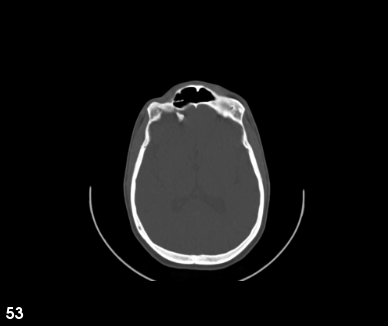
\includegraphics[scale=0.5]{../user_guide_figures/invesalius_screen/text_off.png}
\caption{Exibição de texto desabilitada}
\label{fig:text_off}
\end{figure}
